\documentclass[tikz,border=2pt]{standalone}
\usepackage{amsmath,amssymb}
\usepackage{tikz}
\usetikzlibrary{arrows.meta}

\begin{document}
% The known infinite cardinalities aleph_0 = card(N) and c = card(R) = 2^{aleph_0}; the
% continuum hypothesis asks whether any set has a size strictly in between.
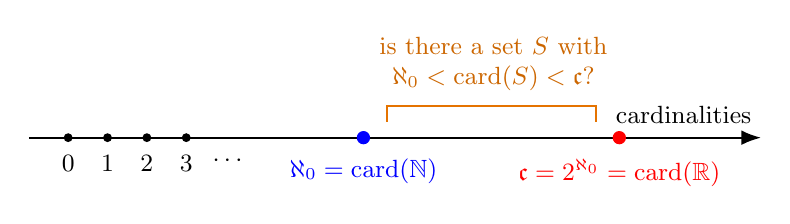
\begin{tikzpicture}[every node/.style={font=\small}, >={Latex[length=2.5mm]}]
	\draw[->, thick] (-0.5,0) -- (8.8,0);
	\node[anchor=south east] at (8.8,0.05) {cardinalities};
	\foreach \x/\l in {0/0, 0.5/1, 1.0/2, 1.5/3} {\fill (\x,0) circle (1.6pt); \node[below=3pt] at (\x,0) {$\l$};}
	\node at (2.05,-0.3) {$\cdots$};
	\fill[blue] (3.75,0) circle (2.4pt);
	\node[blue, below=4pt] at (3.75,0) {$\aleph_0=\operatorname{card}(\mathbb{N})$};
	\fill[red] (7.0,0) circle (2.4pt);
	\node[red, below=4pt] at (7.0,0) {$\mathfrak{c}=2^{\aleph_0}=\operatorname{card}(\mathbb{R})$};
	\draw[orange!90!black, thick] (4.05,0.2) -- (4.05,0.4) -- (6.7,0.4) -- (6.7,0.2);
	\node[orange!80!black, above=2pt, align=center] at (5.4,0.4) {is there a set $S$ with\\ $\aleph_0<\operatorname{card}(S)<\mathfrak{c}$?};
\end{tikzpicture}
\end{document}
